%!TEX root = ../report.tex
\documentclass[../report.tex]{subfiles}
\begin{document}
    \chapter{Evaluation and Results}
	This chapter presents the results of experiments whose implementation details were provided in the last chapter. Besides, the outcomes are systematically analyzed and evaluated.
	
	
	\section{Background}
	We conducted the first three experiments (A. patient-wise attribution map generation, B. composite face generation and C. syndrome-wise attribution map generation) on each of the 139 frequent syndrome classes in the GestaltMatcherDataBase (GMDB) dataset. However, as mentioned earlier, experimental artifacts related to six of the syndromes (Cornelia de Lange syndrome (CDLS), Williams Beuren syndrome (WBS),  Coffin-Siris syndrome (CSS),  Nicolaides-Baraitser syndrome (NBS), Hyperphosphatasia-intellectual disability syndrome or Hyperphosphatasia mental retardation syndrome (HPMRS) and Smith-Lemli-Opitz-Syndrome (SMOS)) were evaluated by an experienced clinical geneticist. The clinician specialized in the diagnosis of three of the syndromes (CDLS, WBS, HPMRS), and had less familiarity with others. Therefore, analyses and discussions on experimental results mostly revolve around the three syndrome categories. Besides, some important findings from other syndromes are also provided. In this section, some background information regarding facial phenotypic features of the syndromes discussed in this chapter is given. 
	
	\subsubsection{Cornelia De Lange Syndrome}
	Cornelia de Lange syndrome (CDLS) is a rare genetic condition present at birth. It is characterized by multiple physical and intellectual abnormalities. There are different variants of the syndrome each identified with its own set of facial features. However, the profile of eyebrows is predominantly considered for diagnosing the syndrome. Figures \ref{fig_cdls_char} and \ref{fig_cdls} show samples contain other facial features related to the genetic condition.
		\begin{figure}[H]
		\centering
		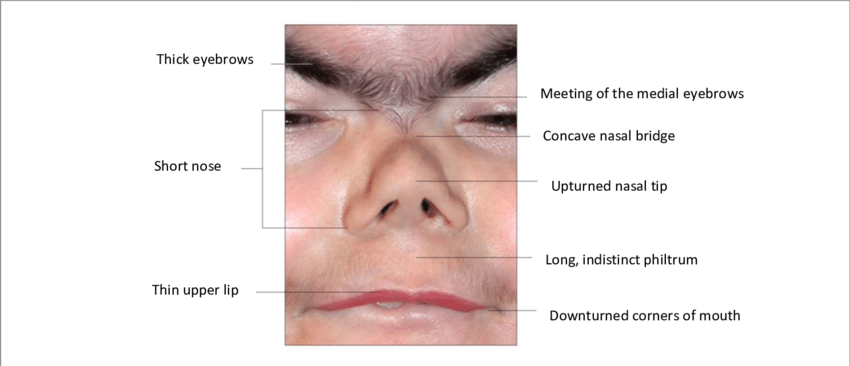
\includegraphics[scale=0.5, trim = 1cm 1cm 1cm 1cm, clip]{chapter6/cdls/cdls_ref.png}	
		\caption[Cardinal features of CDLS]{Cardinal facial features of CDLS. Image source: \cite{kline2018diagnosis}}
		\label{fig_cdls_char}
	\end{figure}
	
	\begin{figure}[H]
		\centering
		\begin{subfigure}[t]{0.24\textwidth}
			\centering
			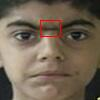
\includegraphics[width=\textwidth]{chapter6/cdls/0_3529.jpg}
			\caption{Synophrys}
		\end{subfigure}
		\begin{subfigure}[t]{0.24\textwidth}
			\centering
			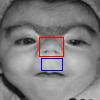
\includegraphics[width=\textwidth]{chapter6/cdls/9_2000.jpg}
			\caption{Depressed nasal bridge (red), long philtrum (blue)}
		\end{subfigure}	
		\begin{subfigure}[t]{0.24\textwidth}
			\centering
			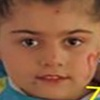
\includegraphics[width=\textwidth]{chapter6/cdls/33_3580.jpg}
			\caption{Thin upper lip}
		\end{subfigure}	
		\begin{subfigure}[t]{0.24\textwidth}
			\centering
			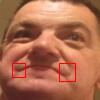
\includegraphics[width=\textwidth]{chapter6/cdls/117_3699.jpg}
			\caption{Down-turned corners of mouth}
		\end{subfigure}
		\caption[Instances of CDLS from GMDB dataset]{Instances of CDLS from GMDB dataset annotated with phenotypic facial features}
		\label{fig_cdls}
	\end{figure}
	
	\subsubsection{Williams Beuren Syndrome}
	Williams Beuren Syndrome (WBS) or Williams syndrome is a rare genetic condition which affects many parts of the human body. The disorder is marked by both prenatal (before birth) and postnatal growth retardation. Flat midface, long philtrum and thick lips are some of the characteristic facial features associated with the syndrome. Refer figures \ref{fig_williams} and \ref{fig_wil_gmdb} contain an animated representative face and examples from GMDB dataset respectively. 
	\begin{figure}[H]\label{fig_williams_char}
	\centering
	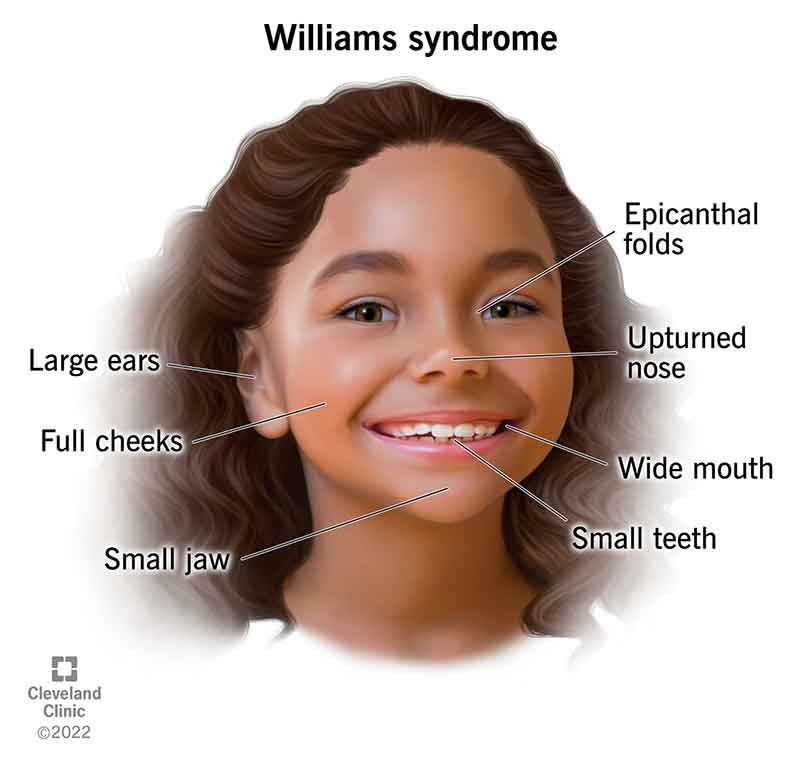
\includegraphics[scale=0.2]{chapter6/william/williams_syndrome_ref.jpg}	
	\caption[An animated characteristic face of WBS]{An animated characteristic face of WBS. Image source: Cleveland clinic \protect\footnotemark.} 
	\end{figure}
	 \footnotetext{Cleveland clinic - \url{https://my.clevelandclinic.org/health/diseases/15174-williams-syndrome}}
	\begin{figure}[H]\label{fig_williams}
		\centering
		\begin{subfigure}[t]{0.24\textwidth}
			\centering
			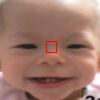
\includegraphics[width=\textwidth]{chapter6/william/4_37.jpg}
			\caption{Depressed nasal bridge}
		\end{subfigure}
		\begin{subfigure}[t]{0.24\textwidth}
			\centering
			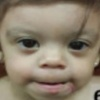
\includegraphics[width=\textwidth]{chapter6/william/4_73.jpg}
			\caption{Long philtrum}
		\end{subfigure}	
			\begin{subfigure}[t]{0.24\textwidth}
			\centering
			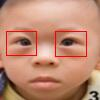
\includegraphics[width=\textwidth]{chapter6/william/130_36.jpg}
			\caption{Puffy eyes}
		\end{subfigure}	
			\begin{subfigure}[t]{0.24\textwidth}
			\centering
			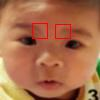
\includegraphics[width=\textwidth]{chapter6/william/164_35.jpg}
			\caption{Medial eyebrow flares}
		\end{subfigure}	
	\caption[Instances of WBS from GMDB dataset]{Instances of WBS from GMDB dataset annotated with phenotypic facial features}
	\label{fig_wil_gmdb}
	\end{figure}





	\subsubsection{Hyperphosphatasia with Mental Retardation Syndrome}
	 
	 \begin{figure}[H]\label{fig_hpmrs}
	 	\centering
	 	\begin{subfigure}[t]{0.17\textwidth}
	 		\centering
	 		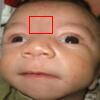
\includegraphics[width=\textwidth]{chapter6/hpmrs/2_499.jpg}
	 		\caption{Hypertelorism}
	 	\end{subfigure}
	 	\begin{subfigure}[t]{0.17\textwidth}
	 		\centering
	 		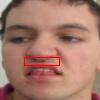
\includegraphics[width=\textwidth]{chapter6/hpmrs/15_1758.jpg}
	 		\caption{Short philtrum}
	 	\end{subfigure}	
	 	\begin{subfigure}[t]{0.17\textwidth}
	 		\centering
	 		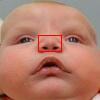
\includegraphics[width=\textwidth]{chapter6/hpmrs/17_1774.jpg}
			\caption{Short nose}
	 	\end{subfigure}	
	 	\begin{subfigure}[t]{0.17\textwidth}
	 		\centering
	 		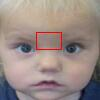
\includegraphics[width=\textwidth]{chapter6/hpmrs/20_888.jpg}
	 		\caption{Broad nasal bridge}
	 	\end{subfigure}	
	 	\begin{subfigure}[t]{0.17\textwidth}
	 		\centering
	 		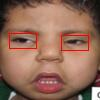
\includegraphics[width=\textwidth]{chapter6/hpmrs/33_1773.jpg}
	 		\caption{Upslanting palpebral fissures}
	 	\end{subfigure}	
	 	\caption[Instances of HPMRS from GMDB dataset]{Instances of HPMRS from GMDB dataset annotated with phenotypic facial features}
	 \end{figure}
	 
	 	\subsubsection{Coffin Siris Syndrome}
	 
	 \begin{figure}[H]\label{fig_cfs}
	 	\centering
	 	\begin{subfigure}[t]{0.17\textwidth}
	 		\centering
	 		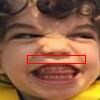
\includegraphics[width=\textwidth]{chapter6/cfs/5_1981.jpg}
	 		\caption{Short philtrum}
	 	\end{subfigure}
	 	\begin{subfigure}[t]{0.17\textwidth}
	 		\centering
	 		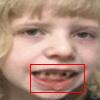
\includegraphics[width=\textwidth]{chapter6/cfs/6_810.jpg}
	 		\caption{Thin upper-lip vermilion and thich lower-lip vermilion }
	 	\end{subfigure}	
	 	\begin{subfigure}[t]{0.17\textwidth}
	 		\centering
	 		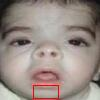
\includegraphics[width=\textwidth]{chapter6/cfs/17_2539.jpg}
	 		\caption{Small chin}
	 	\end{subfigure}	
	 	\begin{subfigure}[t]{0.17\textwidth}
	 		\centering
	 		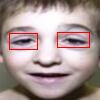
\includegraphics[width=\textwidth]{chapter6/cfs/20_2465.jpg}
	 		\caption{Downslanting palpebral fissures}
	 	\end{subfigure}	
	 	\begin{subfigure}[t]{0.17\textwidth}
	 		\centering
	 		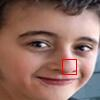
\includegraphics[width=\textwidth]{chapter6/cfs/46_1986.jpg}
	 		\caption{Broad nasal tip}
	 	\end{subfigure}	
	 	\caption[Instances of HPMRS from GMDB dataset]{Instances of CSS from GMDB dataset annotated with phenotypic facial features}
	 \end{figure}
	 
	 
    \section{Experiment A. Patient-wise Attribution Map Generation}
    
    
    
    \subsection{Results from Clinician's Evaluation}
    The clinician was presented with attribution maps of 23 instances from six different syndromes classes in GMDB. However, as mentioned earlier, his specialization was limited to three syndromes which were represented by 15 samples in the questionnaire. Table \ref{tab_cl_acc} shows the sample distribution, and diagnostic performance of the clinician for each syndrome class, without the aid of attribution maps. As described in  Chapter \ref{ch_method}, it is important to note that only samples from the test split of GMDB that were correctly classified by the GestaltMatcher classifier model, were chosen for evaluation. 
    
    
   	\begin{figure}[H]
   	\centering
   	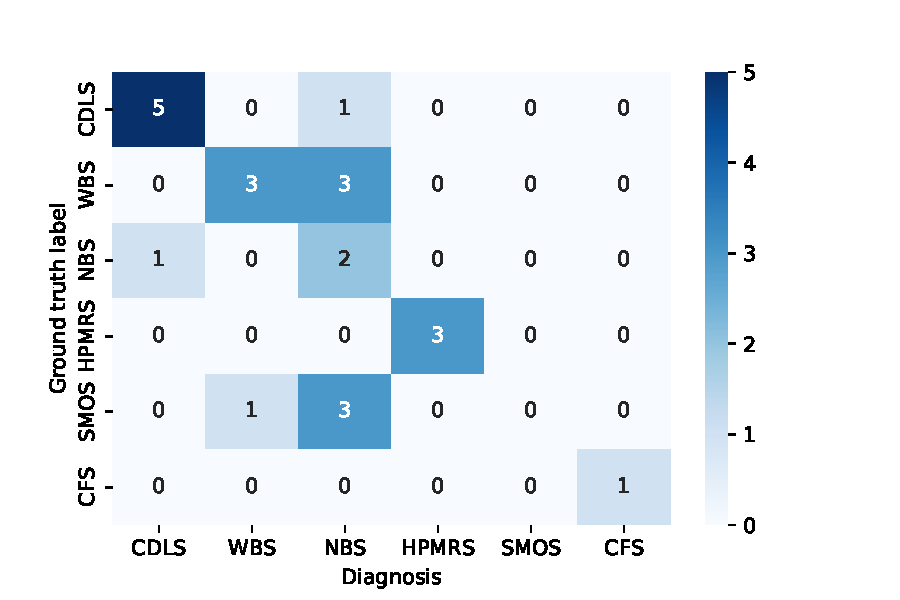
\includegraphics[scale=0.6,trim=0.5cm 0cm 0.5cm 0cm, clip]{chapter6/clinician_conf_matrix.pdf}	
   	\caption[Confusion matrix representing the clinician's
   	diagnostic performance]{Confusion matrix representing the clinician's
   	diagnostic performance}
   \label{fig_clin_perf_mtx} 
   \end{figure}
    

 \begin{table}[H]
 	\begin{tabular}{|c|c|c|c|c|c|c|}
 		\hline
 		\textbf{Syndrome} & \textbf{Sample count} & \textbf{\begin{tabular}[c]{@{}c@{}}Clinician \\ specializes in\\ syndrome\end{tabular}} & \textbf{Precision} & \textbf{Recall} & \multicolumn{1}{l|}{\textbf{F1-score}} & \textbf{Accuracy} \\ \hline
 		\textbf{CDLS}              & 6                     & yes                                                                                     & 0.83               & 0.83            & 0.83                                   & 0.83              \\ \hline
 		\textbf{WBS}               & 6                     & yes                                                                                     & 0.75               & 0.50            & 0.60                                   & 0.50              \\ \hline
 		NBS               & 3                     & no                                                                                      & 0.22               & 0.67            & 0.33                                   & 0.67              \\ \hline
 		\textbf{HPMRS}             & 3                     & yes                                                                                     & 1.00               & 1.00            & 1.00                                   & 1.00              \\ \hline
 		SMOS              & 4                     & no                                                                                      & 0.00               & 0.00            & 0.00                                   & 0.00              \\ \hline
 		CFS               & 1                     & no                                                                                      & 1.00               & 1.00            & 1.00                                   & 1.00              \\ \hline
 	\end{tabular}
 \caption{Diagnostic performance of the clinician on samples in the questionnaire}
  \label{tab_cl_acc}
\end{table}
  \subsubsection{Usefulness of Attribution Maps in Diagnoses}
  Fig \ref{fig_patient_flow} in Chapter \ref{ch_method} enumerated the following possible inferences, which can obtained from responses in the patient-wise attribution map evaluation section of the questionnaire:
  \begin{itemize}
  	\item A. Attribution maps misleads the clinician to make incorrect diagnosis
  	\item B. Attribution maps reinforces the clinician's correct diagnosis
  	\item C. Attribution maps helps the clinician to correct his diagnosis
  	\item D. Attribution maps fail to help the clinician to correct his diagnosis
  \end{itemize} 
  Here, we describe the usefulness of attribution maps and performance of methods used to generate them, by binning clinician responses into one of the above mentioned, and analyzing them. 
  
  As shown in Figure \ref{fig_clin_perf_mtx}, the clinician correctly diagnosed 11 out of the total 15 patient images, presented to him from the syndromes of his specialty, without the aid of attribution maps. His responses to the subsequent questions (Refer questions 2b - 2e in Table \ref{tbl_synd_wise}) asked after the 11 correctly diagnosed cases, indicate that the attribution maps reinforced correct diagnoses (scenario B) in eight cases, and didnot prove helpful (scenario A) in  three. Within the 8 occurrences of scenario B, attribution maps using FullGrad were marked to best highlight the associated facial features in five, followed by the maps of other methods in one each. Among the four misdiagnosed instances, none of the attribution maps proved effective in correcting three of his predictions (scenario D), and a FullGrad attribution map helped him correct one (scenario C). 
  To summarize, the clinician found attribution maps in general to be helpful for diagnosis, in 9 out of 15 instances, and also chose FullGrad maps to highlight relevant facial features in most of the cases.
		\begin{figure}[H]
		\centering			
		\begin{subfigure}[t]{1\textwidth}
			\centering
			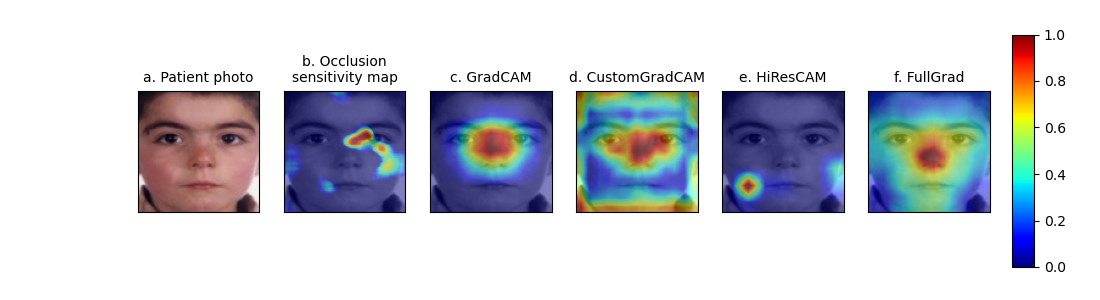
\includegraphics[width=\textwidth, trim = 1cm 2.50cm 1cm 2cm, clip]{chapter6/cdls/0_205.png}
			\caption{Patient with CDLS and eyebrows specified as the key feature}
			\label{sfig_match_1}
		\end{subfigure}
		\begin{subfigure}[t]{1\textwidth}
			\centering
			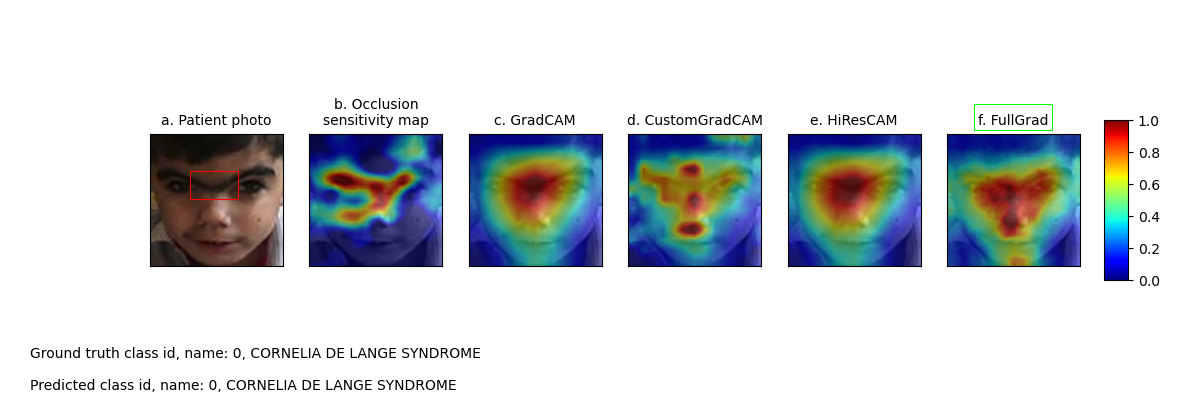
\includegraphics[width=\textwidth, trim = 1cm 2.50cm 1cm 2cm, clip]{chapter6/cdls/4_3556.png}
			\caption{Patient with CDLS and synophrys feature}
			\label{sfig_match_2}
		\end{subfigure}
		\begin{subfigure}[t]{1\textwidth}
			\centering
			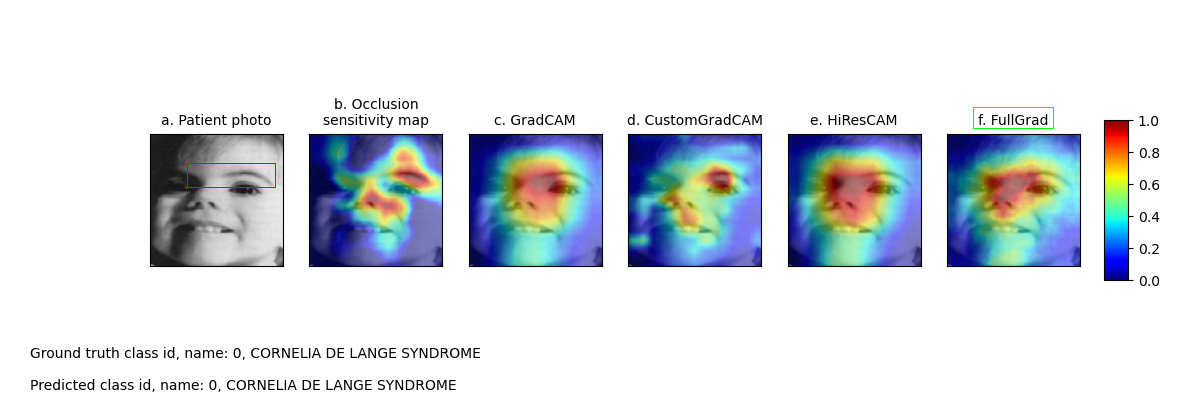
\includegraphics[width=\textwidth, trim = 1cm 2.50cm 1cm 2cm, clip]{chapter6/cdls/6_222.png}
			\caption{Patient with CDLS and eyebrows specified as the key feature}
			\label{sfig_match_3}
		\end{subfigure}
		\begin{subfigure}[t]{1\textwidth}
			\centering
			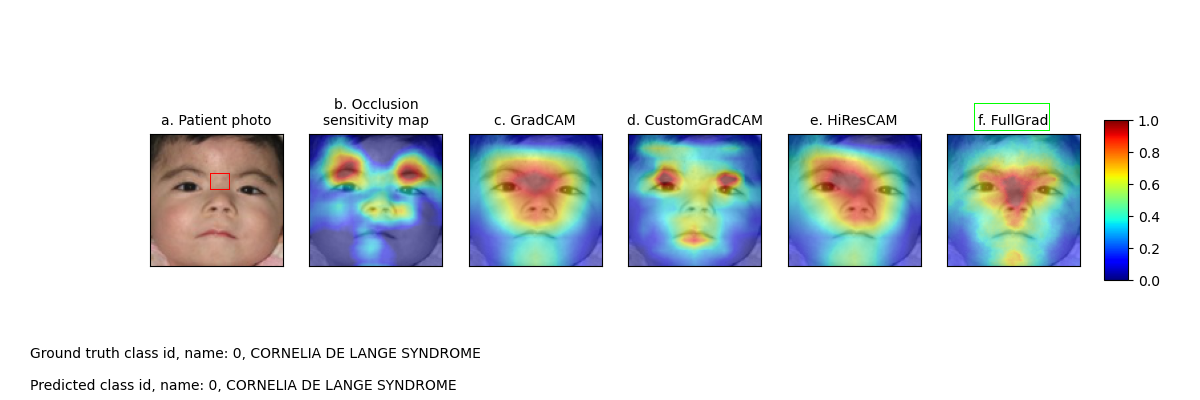
\includegraphics[width=\textwidth, trim = 1cm 2.50cm 1cm 2cm, clip]{chapter6/cdls/7_285.png}
			\caption{Patient with CDLS and nose, depressed nasal bridge reported as the key features}
			\label{sfig_match_4}
		\end{subfigure}
		\begin{subfigure}[t]{1\textwidth}
		\centering
		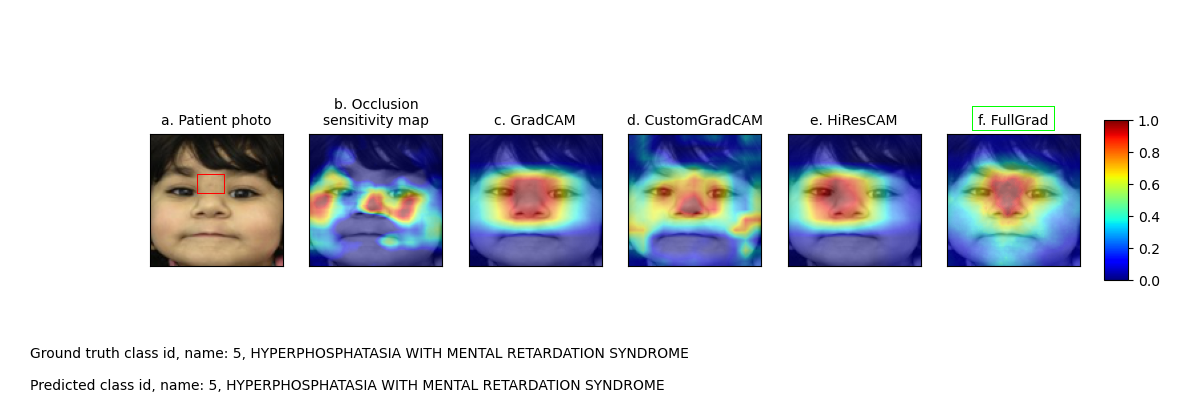
\includegraphics[width=\textwidth, trim = 1cm 2.50cm 1cm 2cm, clip]{chapter6/hpmrs/4_2442.png}
		\caption{Patient with HPMRS and nasal bridge reported as the key feature}
		\label{sfig_match_5}
		\end{subfigure}
		\caption[Attribution maps of instances in which clinician's attention regions matched that of the classifier model]{Attribution maps of instances in which clinician's attention regions matched that of the classifier model. Key features specified and methods chosen by the clinician are boxed in red and green colors respectively}
	\label{fig_match_cl_maps}
	\end{figure}
	\begin{figure}[H]
		\begin{subfigure}[t]{1\textwidth}
			\centering
			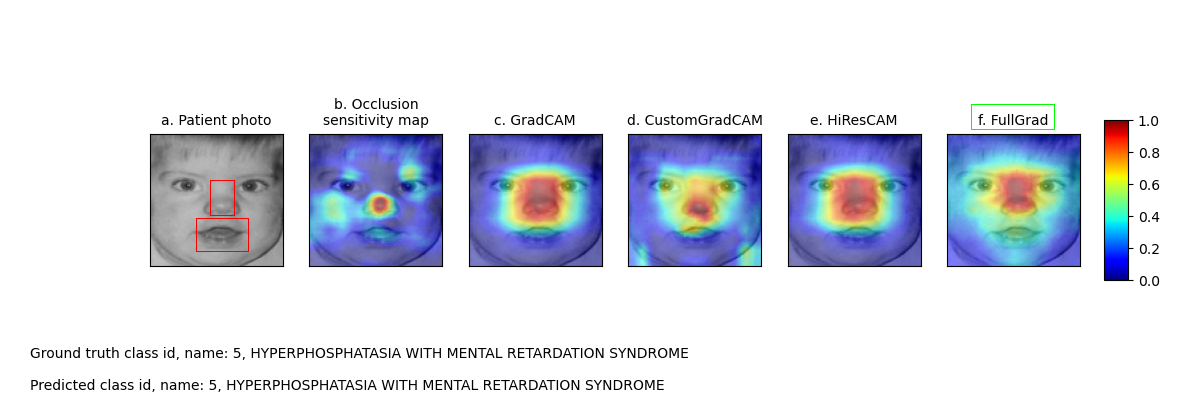
\includegraphics[width=\textwidth, trim = 1cm 2.50cm 1cm 2cm, clip]{chapter6/hpmrs/0_2425.png}
			\caption{Patient with  HPMRS, and nose and mouth specified as key features}
			\label{sfig_diff_1}
		\end{subfigure}
		\begin{subfigure}[t]{1\textwidth}
			\centering
			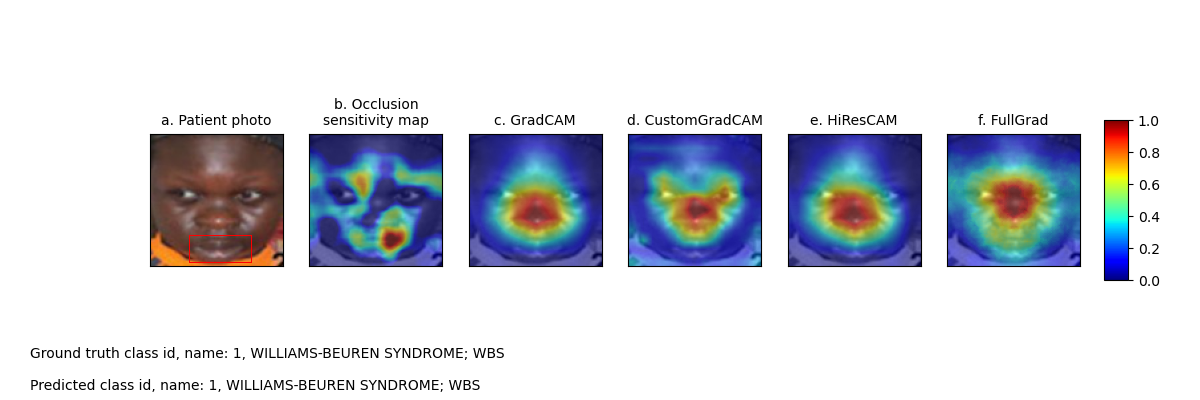
\includegraphics[width=\textwidth, trim = 1cm 2.50cm 1cm 2cm, clip]{chapter6/william/5_31.png}
			\caption{Patient with  WBS, and lips specified as the key feature}
			\label{sfig_diff_2}
		\end{subfigure}
		\begin{subfigure}[t]{1\textwidth}
		\centering
		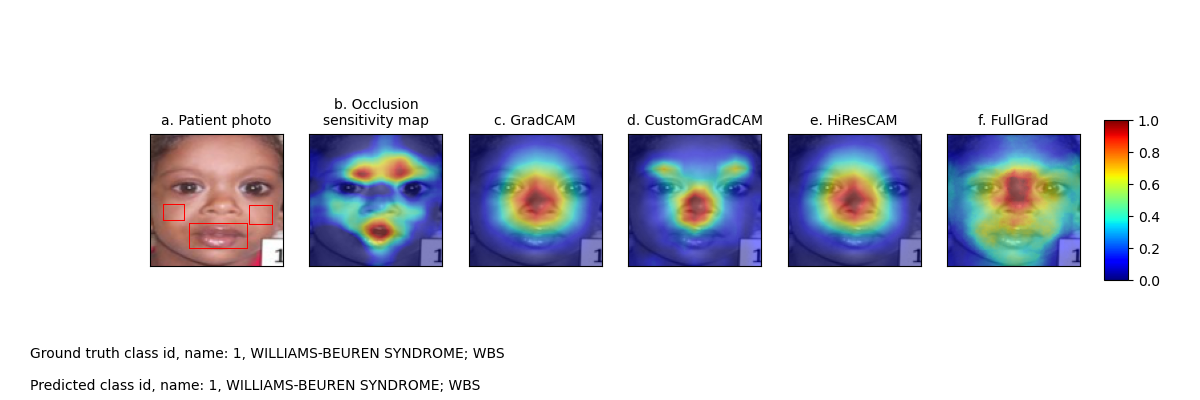
\includegraphics[width=\textwidth, trim = 1cm 2.50cm 1cm 2cm, clip]{chapter6/william/2_137.png}
		\caption{Patient with  WBS, and lips and cheeks specified as key features}
		\label{sfig_diff_3}
		\end{subfigure}
		\begin{subfigure}[t]{1\textwidth}
		\end{subfigure}
		\caption[Attribution maps of instances in which clinician's attention regions differed from that of the classifier model]{Attribution maps of instances in which clinician's attention regions differed from that of the classifier model. Key features specified by the clinician are boxed in red. Method chosen for the first instance is boxed in green color.}
		\label{fig_diff_cl_maps}
	\end{figure}
	\subsubsection{Comparing Attention Regions}
	Besides identifying syndromes and rating attribution maps, the clinician was asked to specify the key facial features which he used for diagnosis (Refer question 2b in \ref{tbl_synd_wise}). From his answers, let us compare his regions of attention with that of the GestaltMatcher classifier model, represented in form of attribution maps.  Figure \ref{fig_match_cl_maps} and Figure \ref{fig_diff_cl_maps}  contain examples of attribution map sets of correctly diagnosed samples, for which features considered crucial by the clinician, matched and differed with that of the classifer respectively.\\
	He reported the eyebrow region to contain key features for diagnosing CDLS, in most of the cases, especially the occurrence of synophrys such as found in figures \ref{sfig_match_1} and \ref{sfig_match_2}. Besides, features in the nose region such as the depressed nasal bridge (refer Figure \ref{sfig_match_5}) were also considered important for his identification. Attribution maps generated using FullGrad were reported to correctly highlight key features of CDLS in three out of six cases, followed by GradCAM in two. The clincial geneticist found none of the maps to be helpful in diagnosing one instance. On the whole, attribution maps were found to be helpful in diagnosing CDLS.\\
	In the case of HPMRS samples, nose and mouth regions were pointed out to contain the syndrome's characteristic features (refer figures \ref{sfig_match_5} and \ref{sfig_diff_1}). FullGrad maps are reported to highlight the characteristic nose region in most of the cases. However, none of the maps highlighted the mouth feature, as it can observed from  Figure \ref{sfig_diff_1}.\\
    Samples presented from WBS were reported to contain key facial features in lip and cheek regions of the face (refer figures \ref{sfig_diff_2} and \ref{sfig_diff_3}). Analyzing clinician responses pertaining the syndrome reveal that none of attribution maps proved helpful for him, both in cases of reinforcing correct diagnoses and correcting misdiagnoses. More importantly, it can be observed that the maps highlighted the nose region, a feature that is not characteristic of the syndrome. However, regions highlighted in occlusion sensitivity maps contain features that were considered by the clinician. This finding raised doubts on faithfulness \footnote[1]{Accurate representation of the reasoning process behind a model's prediction} of the considered attribution methods. Therefore, we attempted to understand the cause of the issue by visualizing and analyzing layer-wise activation maps of different samples.
    
    \subsubsection{Layer-wise Activation Visualization and Analysis}
    We generated attribution maps for all ten convolutional layers of the classifier model using GradCAM and HiResCAM methods. This was done to check whether the missing features get highlighted in attributions of layers other than what were chosen for the experiment. We chose conv\_9 for GradCAM and HiResCAM, and conv\_6, conv\_7 and conv\_9 to generate maps using CustomGradCAM. FullGrad is a layer agnostic approach, and therefore was excluded.\\
	Figure \ref{fig_layer_quest} contains layer-wise visualizations for samples whose attribution maps failed to highlight the key facial features. The first pair of visualizations correspond to the image in Figure \ref{sfig_diff_1} whose maps failed to highlight the mouth region. The area gets highlighted in the conv\_7 layer visualization using GradCAM. Likewise, incases of visualizations of WBS samples (refer second and third pair of rows in Figure \ref{fig_layer_quest}), the key features in lip and cheek regions get highlighted in other convolutional layers.\\
	We extended this analysis to samples in WBS which were not included in the questionnaire. This was performed to find whether visualizations of any particular layer or set of layers highlighted  key features in all instances. Figure \ref{fig_layer_gmdb} contain visualizations of three of such samples, whose key features are in the lip region. The region was found to be highlighted in visualizations of different layers in different samples. This inconsistent behavior of attribution methods poses a challenge in using them to explain GestaltMatcher predictions in a clinical setting.  
    \begin{sidewaysfigure}
    	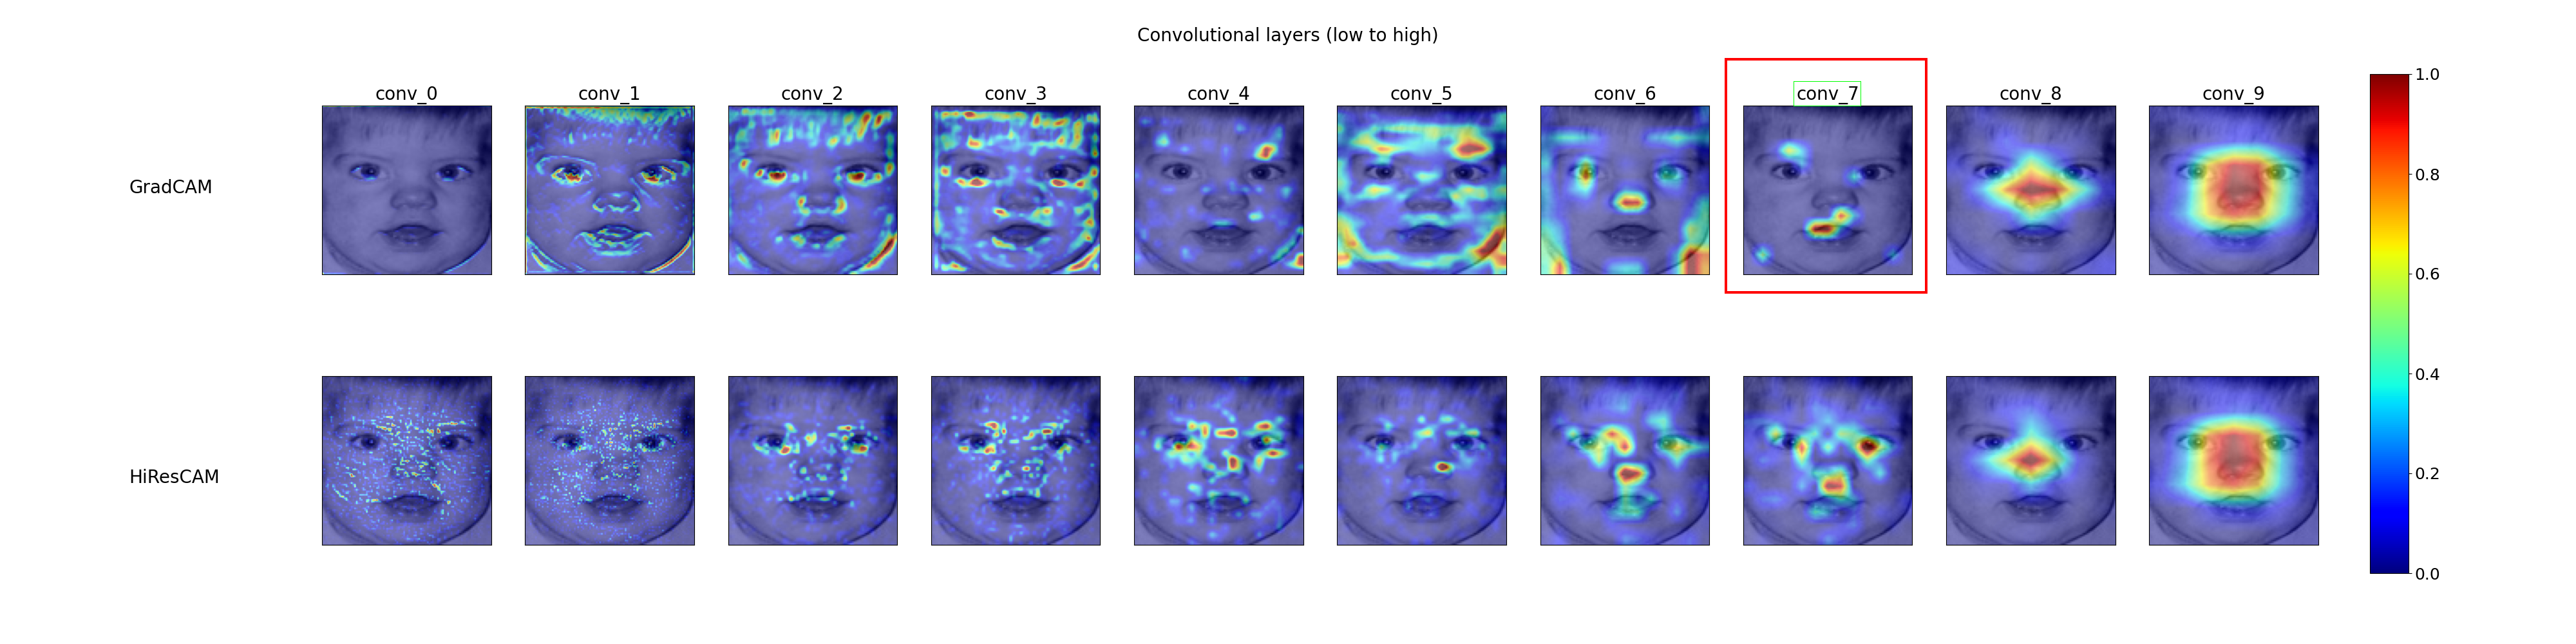
\includegraphics[scale=0.22, trim = 1cm 2cm 1cm 2cm, clip]{chapter6/hpmrs/0_2425_layer.png}
    	
    	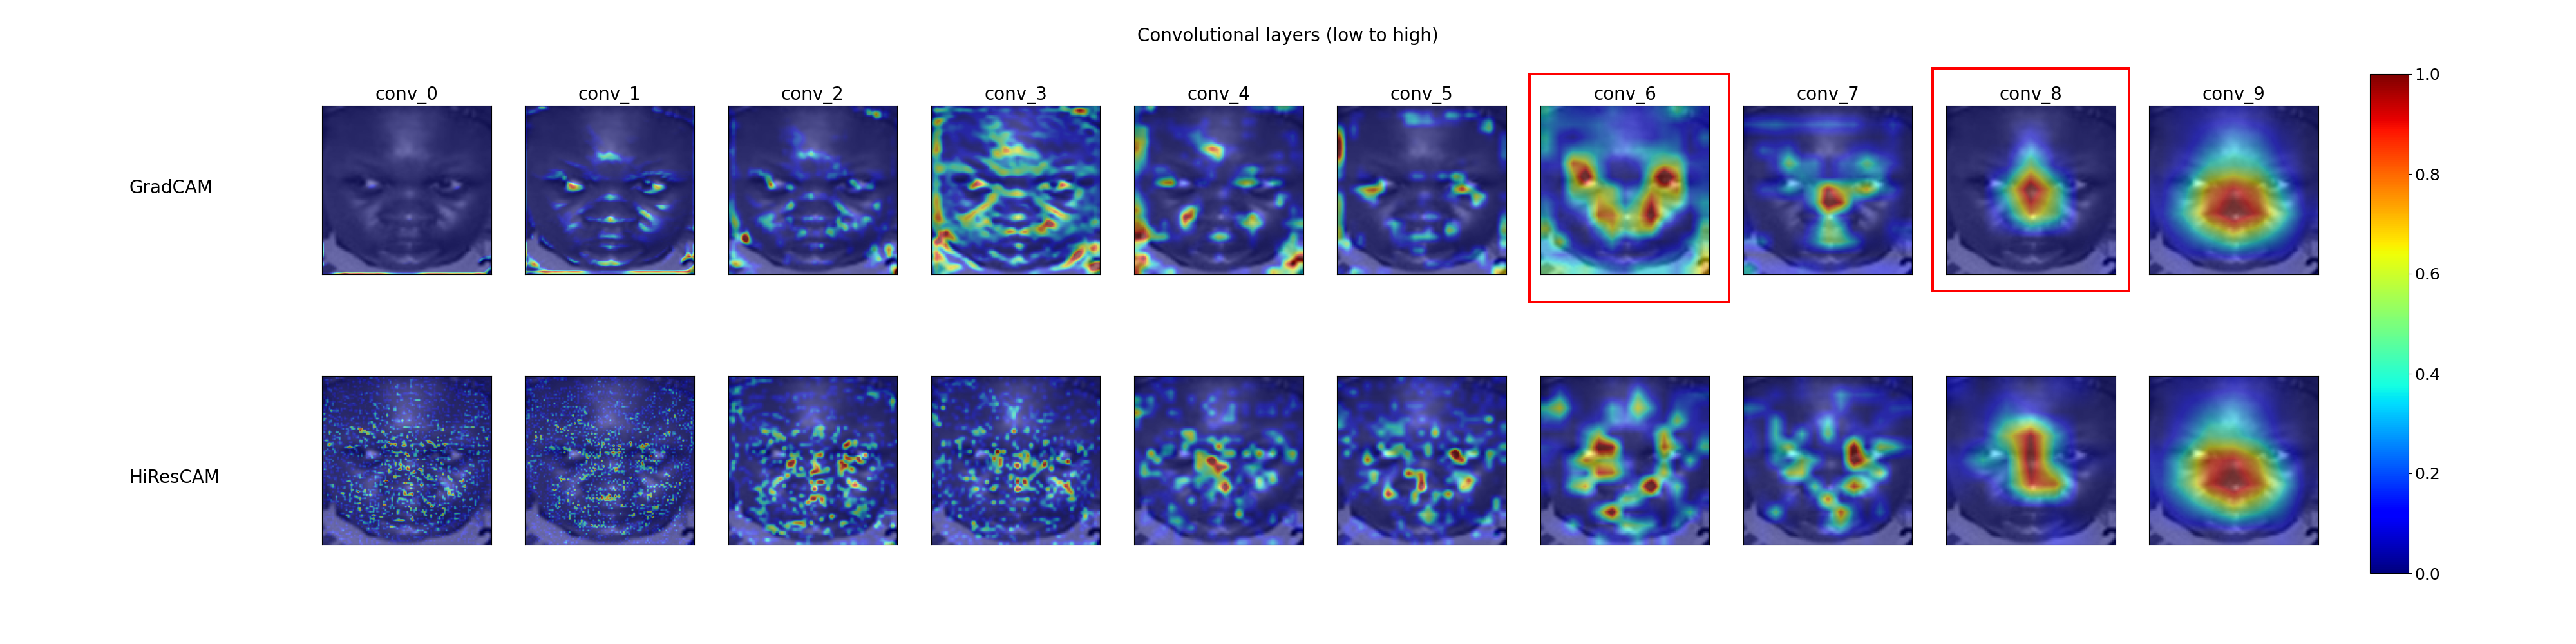
\includegraphics[scale=0.22, trim = 1cm 2.50cm 1cm 2.50cm, clip]{chapter6/william/5_31_layer.png}
	      
    	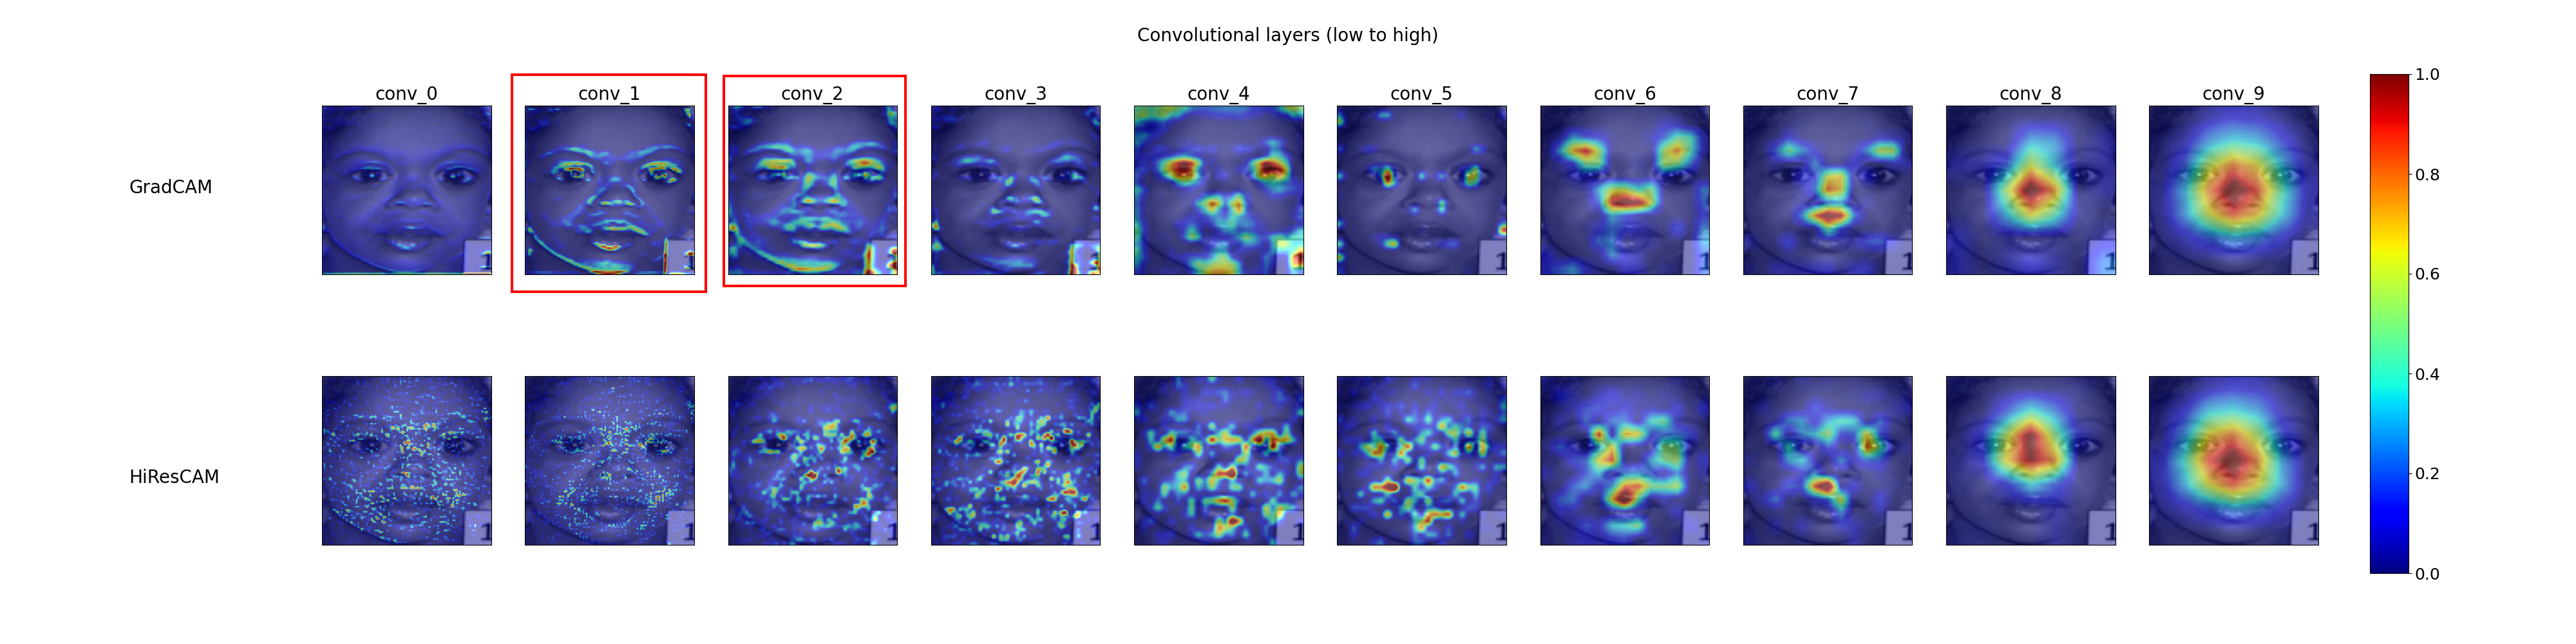
\includegraphics[scale=0.22, trim = 1cm 2.50cm 1cm 2.50cm, clip]{chapter6/william/2_137_layer.png}
    	\caption[Example layer-wise activation map visualizations for instances presented in the questionnaire]{Example layer-wise activation map visualizations for instances presented in the questionnaire. Layers highlighting syndromic features are boxed in red.}
	   \label{fig_layer_quest}	
    \end{sidewaysfigure}

	\begin{sidewaysfigure}
		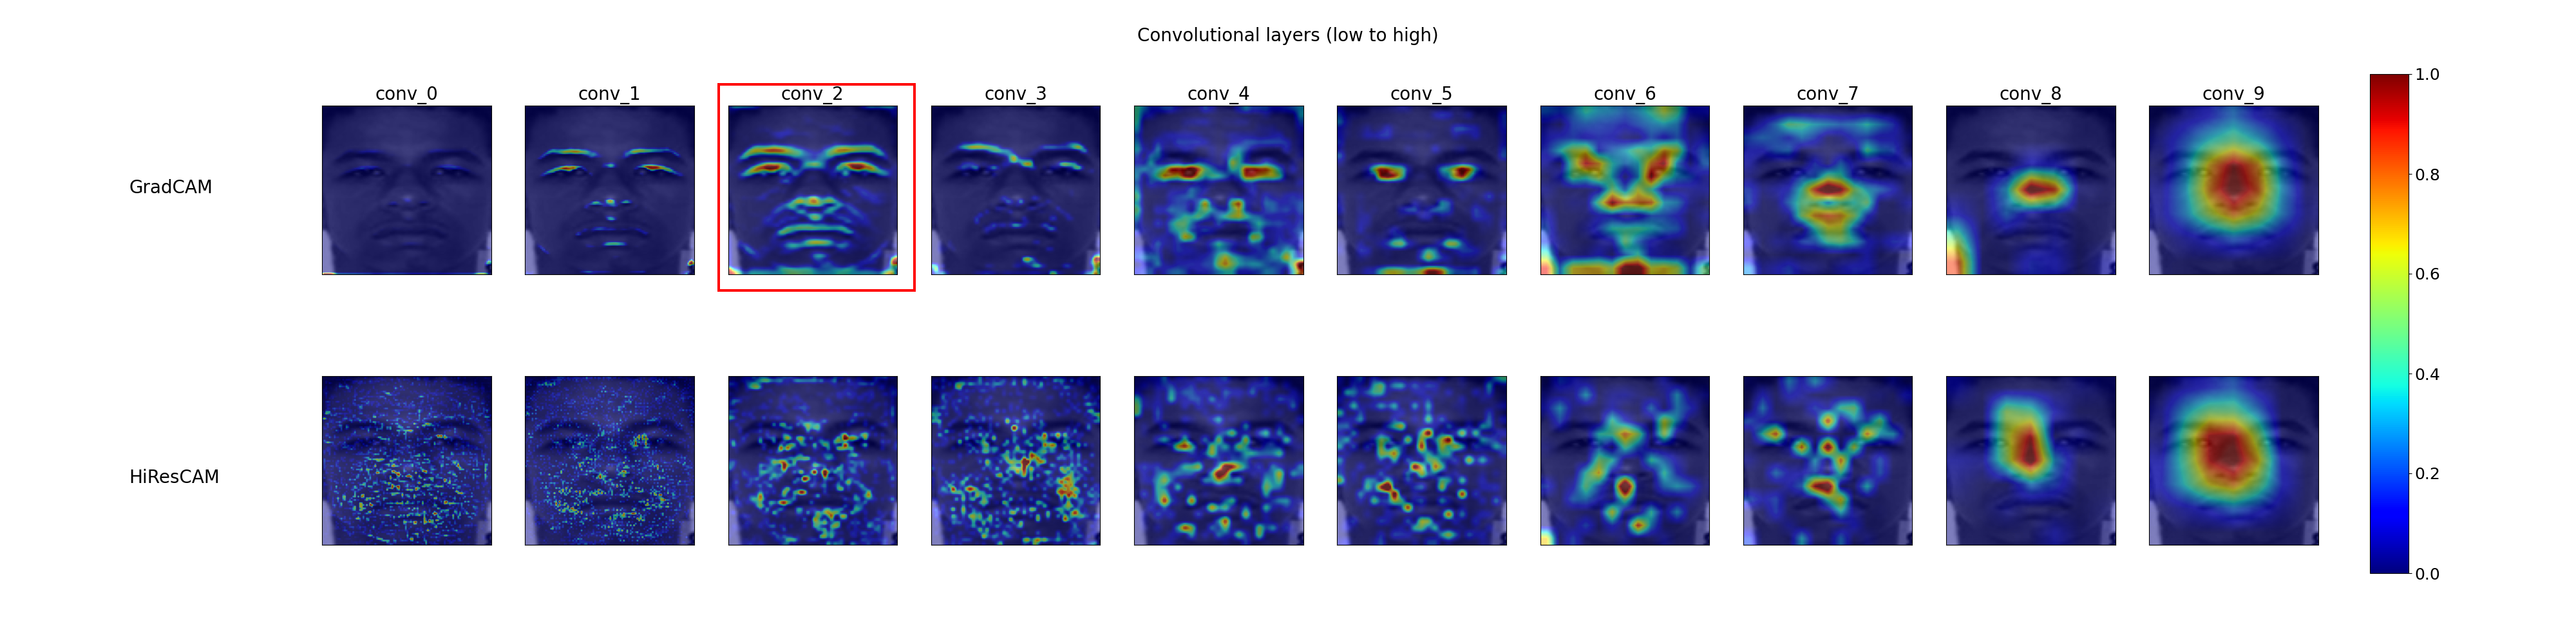
\includegraphics[scale=0.22, trim = 1cm 2.50cm 1cm 2.50cm, clip]{chapter6/william/20_95_layer.png}		
		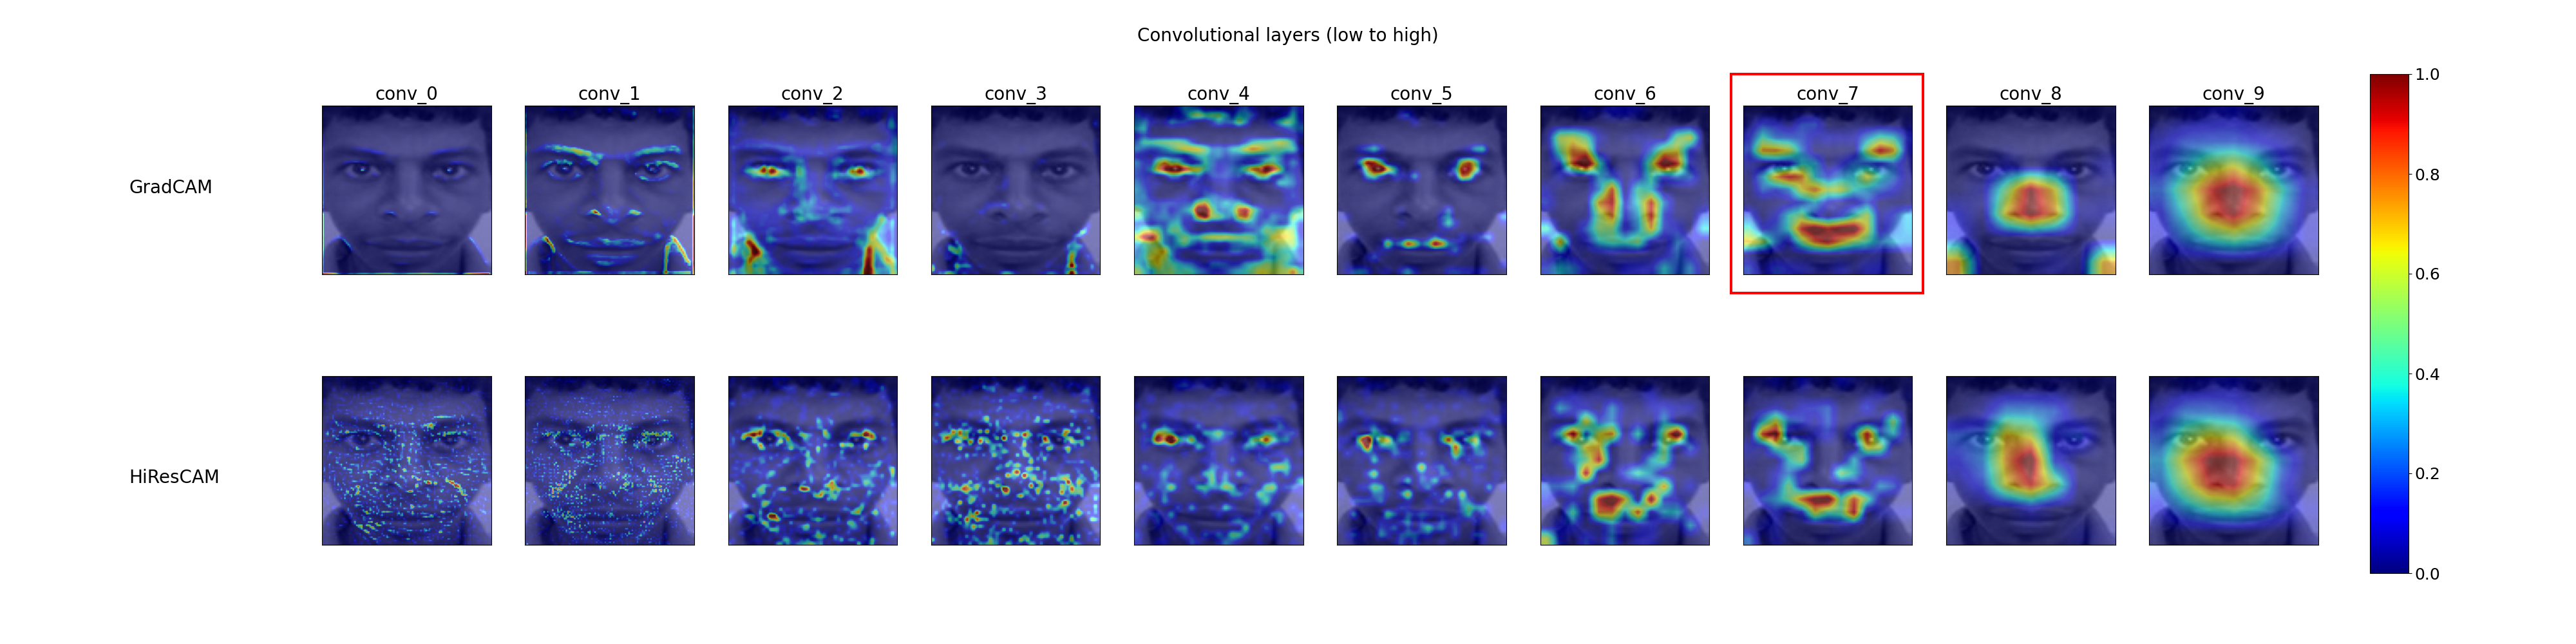
\includegraphics[scale=0.22, trim = 1cm 2.50cm 1cm 2.50cm, clip]{chapter6/william/16_3632_layer.png}
		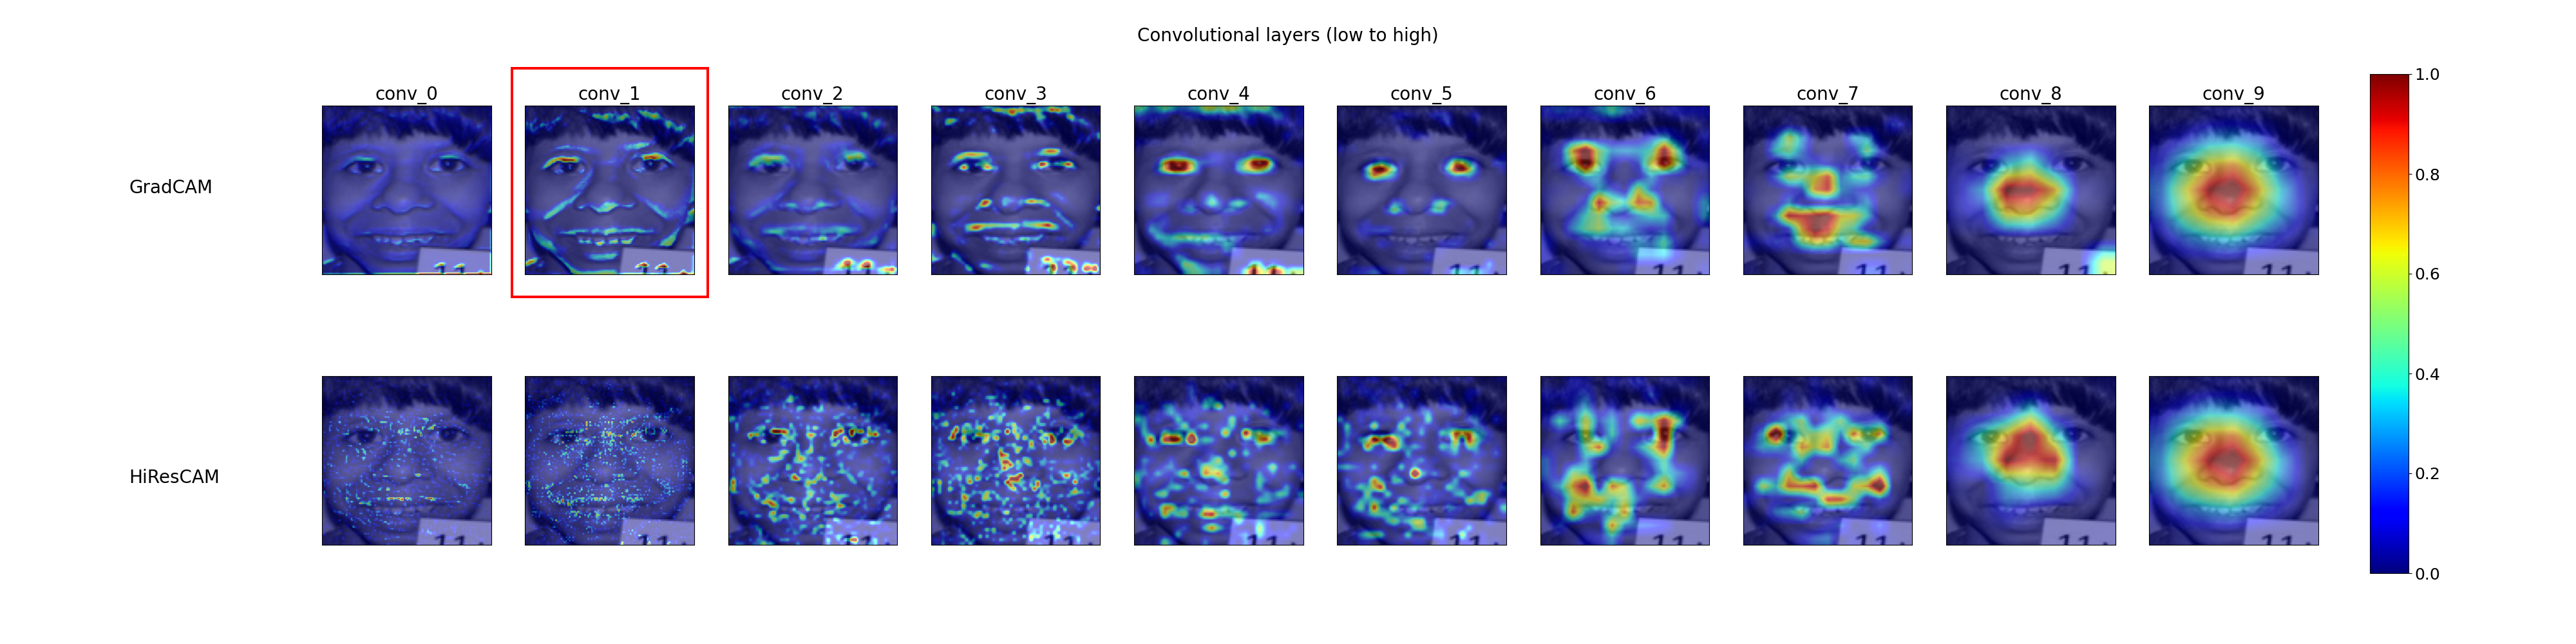
\includegraphics[scale=0.22, trim = 1cm 2.50cm 1cm 2.50cm, clip]{chapter6/william/14_142_layer.png}
		\caption[Example layer-wise activation map visualizations for instances not present in the questionnaire but in GMDB dataset]{Example layer-wise activation map visualizations for instances not present in the questionnaire but in GMDB dataset. Layers highlighting syndromic features are boxed in red.}
		\label{fig_layer_gmdb}
	\end{sidewaysfigure}

	\subsection{Qualitative Evaluation}
  
    \subsection{Evaluation Summary}
    \pagebreak
    \section{Experiment B. Composite Face Generation}
    A composite face provides a characteristic representation of the facial phenotype of a given genetic
    syndrome. Figure \ref{fig_comp_gmdb} contains composite faces of the twelve largest classes of the GMDB dataset. 
       \begin{figure}[H]
    	\begin{subfigure}[t]{0.45\textwidth}
    		\centering
    		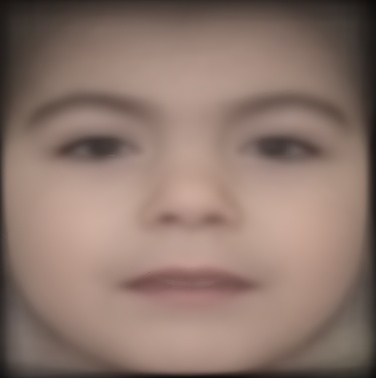
\includegraphics[scale=0.4]{chapter6/cfaces/0.jpg}
    		\caption{Cornelia de Lange syndrome}    		
    	\end{subfigure}
    	\begin{subfigure}[t]{0.45\textwidth}
    		\centering
    		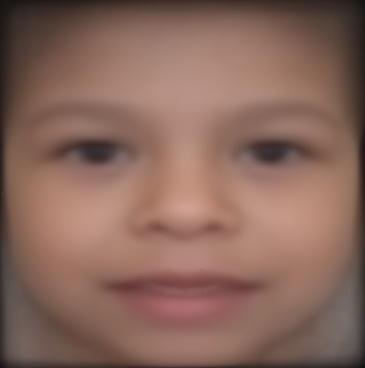
\includegraphics[scale=0.4]{chapter6/cfaces/1.jpg}
    		\caption{Williams syndrome}   		
    	\end{subfigure}
    	\begin{subfigure}[t]{0.45\textwidth}
    		\centering
    		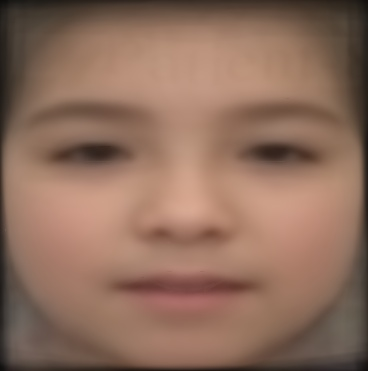
\includegraphics[scale=0.4]{chapter6/cfaces/2.jpg}
    		\caption{Wiedemann-Steiner syndrome}    	
    	\end{subfigure}
    \begin{subfigure}[t]{0.45\textwidth}
    	\centering
    	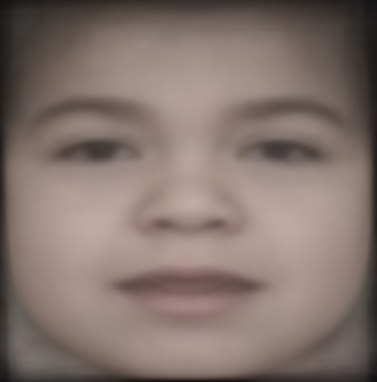
\includegraphics[scale=0.4]{chapter6/cfaces/3.jpg}
    	\caption{Mucopolysaccharidoses}
    \end{subfigure}
	\begin{subfigure}[t]{0.45\textwidth}
		\centering
		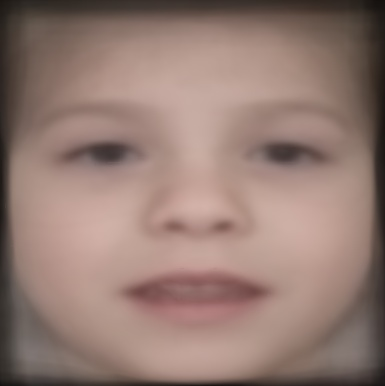
\includegraphics[scale=0.4]{chapter6/cfaces/4.jpg}
		\caption{Nicolaides-Baraitser syndrome}
	\end{subfigure}
	\hspace{1.5cm}
	\begin{subfigure}[t]{0.45\textwidth}
		\centering
		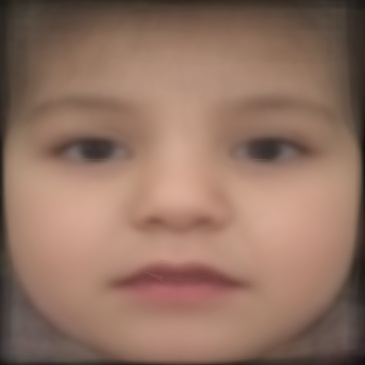
\includegraphics[scale=0.4]{chapter6/cfaces/5.jpg}
		\caption{Hyperphosphatasia with mental retardation syndrome}
	\end{subfigure}
	\end{figure}
	\begin{figure}[H]\continuedfloat
		\begin{subfigure}[t]{0.45\textwidth}
			\centering
			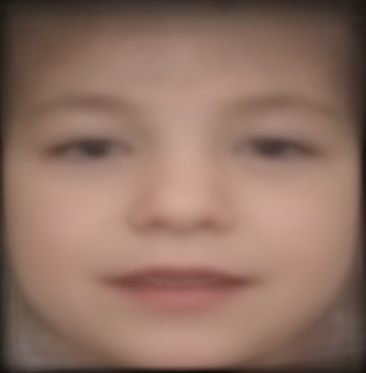
\includegraphics[scale=0.4]{chapter6/cfaces/6.jpg}
			\caption{Baraitser-Winter syndrome}
		\end{subfigure}
		\begin{subfigure}[t]{0.45\textwidth}
			\centering
			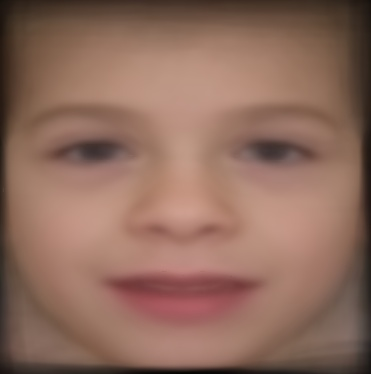
\includegraphics[scale=0.4]{chapter6/cfaces/7.jpg}
			\caption{Smith-Lemli-Opitz syndrome}
		\end{subfigure}
		\begin{subfigure}[t]{0.45\textwidth}
			\centering
			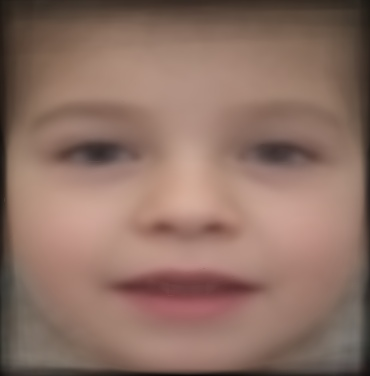
\includegraphics[scale=0.4]{chapter6/cfaces/8.jpg}
			\caption{Coffin-Siris syndrome}
		\end{subfigure}
		\hspace{1.5cm}
		\begin{subfigure}[t]{0.45\textwidth}
			\centering
			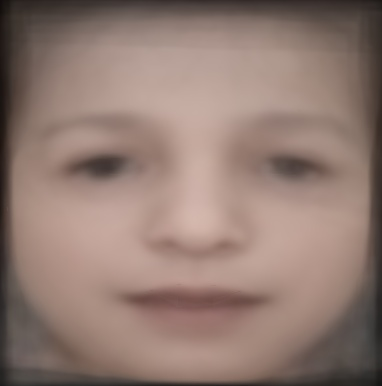
\includegraphics[scale=0.4]{chapter6/cfaces/9.jpg}
			\caption{Treacher Collins syndrome}
		\end{subfigure}
			\begin{subfigure}[t]{0.45\textwidth}
		\centering
		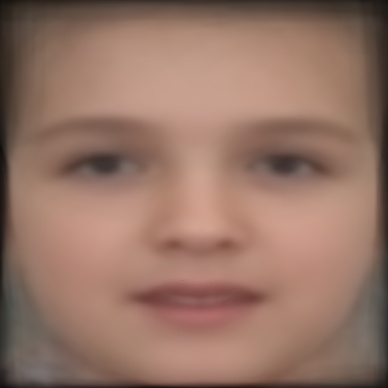
\includegraphics[scale=0.4]{chapter6/cfaces/10.jpg}
		\caption{Sotos syndrome}
	\end{subfigure}
	\hspace{1.5cm}
	\begin{subfigure}[t]{0.45\textwidth}
		\centering
		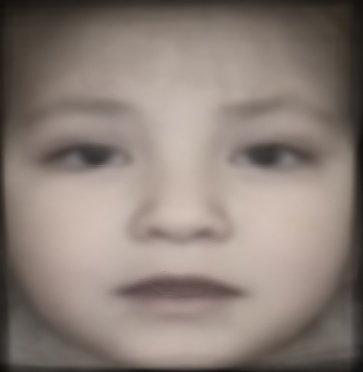
\includegraphics[scale=0.4]{chapter6/cfaces/11.jpg}
		\caption{Kabuki syndrome}
	\end{subfigure}
	\caption{Composite faces of the twelve largest syndrome classes in GMDB dataset}
	\label{fig_comp_gmdb}
\end{figure}

\begin{figure}[H]
	\centering
	\begin{subfigure}[t]{0.8\textwidth}
		\centering
		\hspace{-0.5cm}
		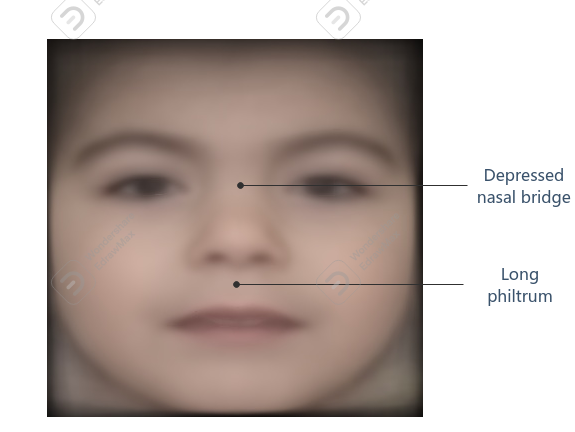
\includegraphics[scale=0.53]{chapter6/cfaces/0_labeled.png}
		\caption{Composite face of CDLS labeled with phenotypic features}
	\end{subfigure}
	\begin{subfigure}[t]{0.8\textwidth}
		\centering
		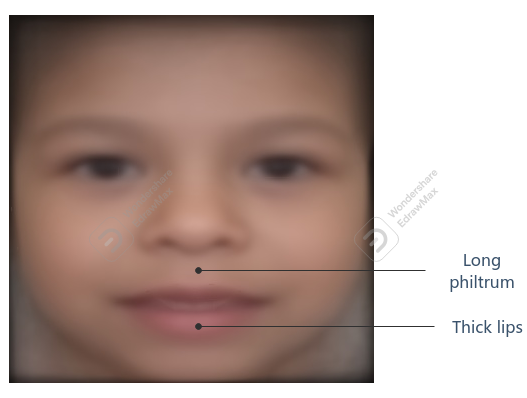
\includegraphics[scale=0.53]{chapter6/cfaces/1_labeled.png}
		\caption{Composite face of WBS labeled with phenotypic features}
	\end{subfigure}
	\begin{subfigure}[t]{0.8\textwidth}
		\centering
		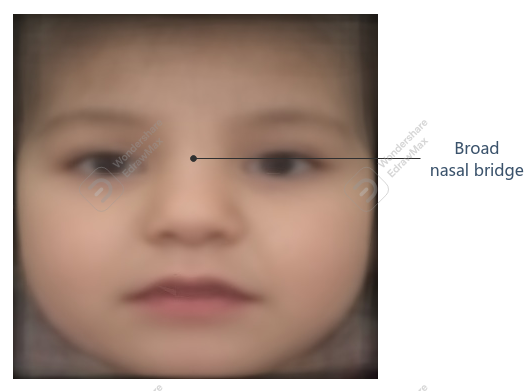
\includegraphics[scale=0.53]{chapter6/cfaces/5_labeled.png}
		\caption{Composite face of HPMRS labeled with feature}
		\label{sfig_diff_3}
	\end{subfigure}
	\caption{Composite faces of the syndromes evaluated by the clinician labeled with phenotypic features}
	\label{fig_comp_lab}
\end{figure}
Similar to other experimental artifacts, the clinician evaluated composite faces representing six syndromes. He found all three faces pertaining syndromes he specialized (CDLS, WBS, HPMRS), to contain their respective characteristic features. The same was reported for SMOS, although he was not experienced in diagnosing the syndrome. We observed the presence of a few though not all distinctive facial features in composite faces of CDLS, WBS and HPMRS (Refer Figure \ref{fig_comp_lab}). The absence of other characteristic features can be attributed to the fact that composite faces were generated by averaging variations in their constituent images. Besides acting as an input artifact for syndrome-wise attribution map generation, composite faces can serve as reference images for clinicians.

    \section{Experiment C. Syndrome-wise Attribution Map Generation}
    
    
    
    
    
    
        \begin{sidewaysfigure}
    	\includegraphics[scale=0.5]{chapter6/syndrome_maps/0.png}
    	
    	\includegraphics[scale=0.5]{chapter6/syndrome_maps/1.png}
    	
    	\caption[Example layer-wise activation map visualizations for instances presented in the questionnaire]{Example layer-wise activation map visualizations for instances presented in the questionnaire. Layers highlighting syndromic features are boxed in red.}
    	\label{fig_layer_quest}	
    	\end{sidewaysfigure}
    
            \begin{sidewaysfigure}
    	\includegraphics[scale=0.5]{chapter6/syndrome_maps/5.png}
    	    	\includegraphics[scale=0.5]{chapter6/syndrome_maps/8.png}
    	
    	\caption[Example layer-wise activation map visualizations for instances presented in the questionnaire]{Example layer-wise activation map visualizations for instances presented in the questionnaire. Layers highlighting syndromic features are boxed in red.}
    	\label{fig_layer_quest}	
    \end{sidewaysfigure}
    
    
 
%	\begin{figure}[H]
%		\centering
%		\begin{subfigure}[t]{0.8\textwidth}
%			\centering
%			\hspace{-0.5cm}
%			\includegraphics[scale=0.53]{chapter6/syndrome_maps/0.pdf}
%			\caption{Composite face of CDLS labeled with phenotypic features}
%		\end{subfigure}
%		\begin{subfigure}[t]{0.8\textwidth}
%			\centering
%			\includegraphics[scale=0.53]{chapter6/syndrome_maps/1.pdf}
%			\caption{Composite face of WBS labeled with phenotypic features}
%		\end{subfigure}
%	\end{figure}
%
%
%		\begin{figure}[H]
%		\centering
%		\begin{subfigure}[t]{0.8\textwidth}
%			\centering
%			\hspace{-0.5cm}
%			\includegraphics[scale=0.53]{chapter6/syndrome_maps/0.pdf}
%			\caption{Composite face of CDLS labeled with phenotypic features}
%		\end{subfigure}
%		\begin{subfigure}[t]{0.8\textwidth}
%			\centering
%			\includegraphics[scale=0.53]{chapter6/syndrome_maps/1.pdf}
%			\caption{Composite face of WBS labeled with phenotypic features}
%		\end{subfigure}
%	\end{figure}




	\section{Experiment D. Dataset Imbalance - Explanation Quality Analysis}

    \section{Evaluation Summary}


\end{document}
